\documentclass[12pt, a4paper]{article}
\usepackage[utf8]{inputenc}
\usepackage{amsmath}
\usepackage{amssymb}
\usepackage{natbib}
\usepackage{mathtools}
\usepackage{titling}
\usepackage[hidelinks]{hyperref}
\usepackage{booktabs}
\usepackage{float}
\usepackage{pbox}
\usepackage{adjustbox}
\usepackage{MnSymbol}
\usepackage{wasysym}
\usepackage{geometry}
\usepackage{ragged2e}
\usepackage{appendix}
\usepackage[table]{xcolor} 
\usepackage[group-separator={,}, round-mode = places, round-precision = 2]{siunitx}

\usepackage{setspace}
\doublespacing

\usepackage {tikz}
\usetikzlibrary{arrows}
\usetikzlibrary{shapes.misc, positioning, shapes.geometric}

\usepackage[font={it}, labelfont=bf]{caption}
\usepackage{graphicx}

\graphicspath{{../images/}}

\author{Reid McIlroy-Young}
\title{Data Visualization: Final project\\RNN Occlusion visualization}
\date{June, 2018}

\setcounter{tocdepth}{2}

\begin{document}
\maketitle
\section*{Introduction}
	
The existing work on visualization of of recurrent neural networks (RNN) is quite lacking, the best I am aware of is a sequence to sequence and word/character model visualizer that uses a parallel coordinates plot: \href{http://lstm.seas.harvard.edu/client/index.html}{lstm.seas.harvard.edu/client/index.html}. This is a visual of how the Long Short Term Memory (LSTM) layers are working but is busy, complex and unintuitive. There have been a few other pieces of work done on the topic, mostly focusing on sequence to sequence or generative models, but none on classifiers that I could find. The goal of this project is get a better visualizer of of LSTM/RNN classifiers as that is what I am using in my work.

For this project I limited my scope to a single pre-trained RNN, the RNN reads social science papers an assess how computational they are, with positive $1$ being very and negative $0$ being not at all. It does this by reading the papers abstract and title which have been converted to a sequence of word2vec vectors after standard tokenization and normalization (i.e. regex based tokenizing). Internally there are 8 LSTM sections four for the title and four for the abstract with two stacked and reading forward and the other two stacked and reading backwards. Then the final outputs are combined by a single layer of neurons.

\section*{Methods}

The first attempt I made was looking at the activations of the RNN, Figure \ref{acts}, tries to show the activations at each word that were fed to the single layer before being converted to a binary output. Note, that in main usage and training only the last output is used. This display has numerous problems, first of which is that it is attempting to display $512 \times $ the number of words, floating point values and has no good way of relating them spatially as column 1 and 2 could be just as related as columns 1 and 400 so the x-axis is categorical, but the scale is too small for this to be obvious. Additionally the magnitude of the activation is not guaranteed to correlate with significance, so this display is even more fundamentally flawed.
	
\begin{figure}[ht]
	\centering
	\begin{adjustbox}{center}
		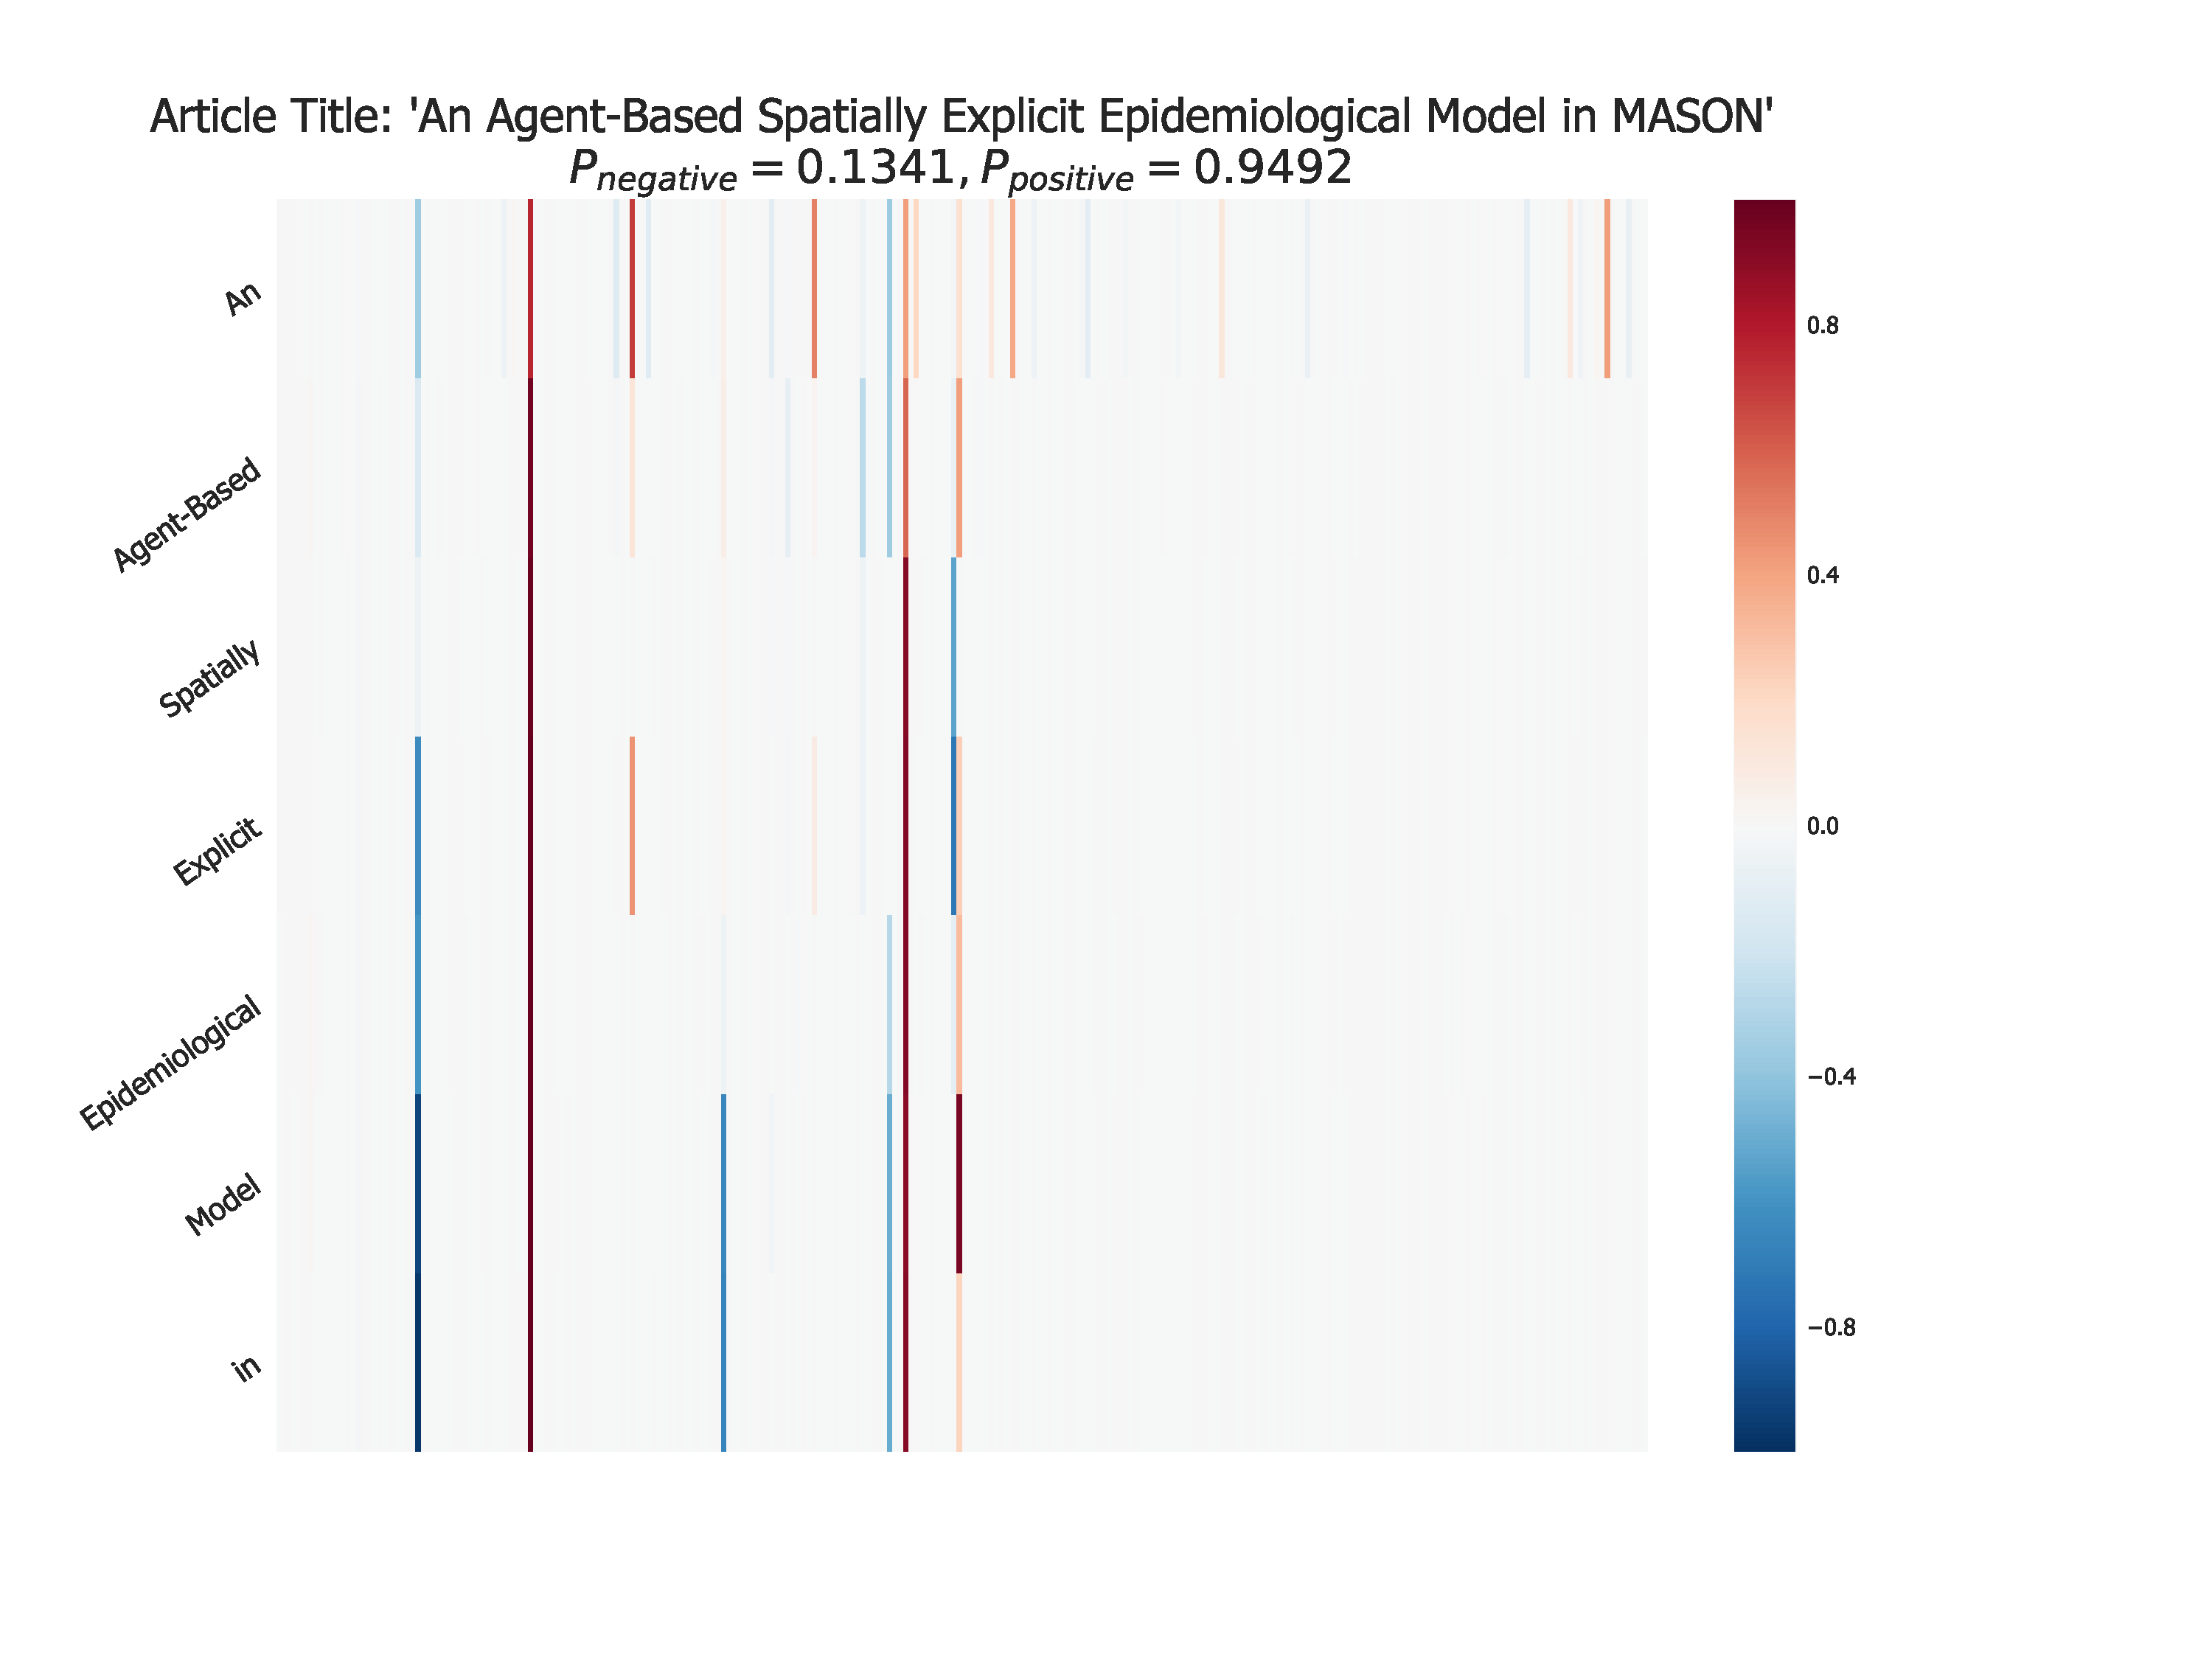
\includegraphics[width=1\textwidth]{activations}
	\end{adjustbox}
	\caption{Example of output activations for a positive example}\label{acts}
\end{figure}

The second attempt I made is at mapping NN with each neuron a node in a graph and each connection an edge. This had many issues, first the number of edges is huge, so the network appears to be a hairball, unless carefully laid out and second once laid out nothing is visible since the layout must be huge. My solution to this was to plot the nodes and edges on a map, but this failed as there is not really a good way of doing it in R. I think this is still worth considering but right now is non-trivial.

The third attempt was inspired by work done in convolutional neural networks (CNNs). CNNs often have a direct visual interpretation since they are based on naturally occurring neural structures for processing images. A method used to some success in convolutional neural network (CNN) visualization and introspection is the \textit{occlusion experiment}, where an image is broken into subsections and the CNN is asked to make a classification with the subsection removed. This method allows one to measure the significance of each of the subsections by measuring how their removal affects the classification certainty. Figure \ref{oc1} shows the effects of removing words from the title and abstract on the classification probability for a toy example with the title of \textit{Exploration of humans, society and R} and abstract `\textit{We used methods and techniques to do stuff. Weber Freud and vocabulary acquisition were explored. Then we did more stuff. Our code can be found on Github.}'. We can see in the bottom left that if the title is \textit{Exploration} and the abstract simply \textit{We used methods and techniques to do stuff.} then the full model gives it a $0.64$ probability of being computational, but if you add the sentence \textit{Weber Freud and vocabulary acquisition were explored.} the probability drops to $0.41$. Similarly adding the final sentence \textit{Our code can be found on Github.} firmly puts the record as computational with a probability of $0.89$ and if \textit{R} is added to the title, the probability goes up to $0.95$.
	
\begin{figure}[ht]
	\centering
	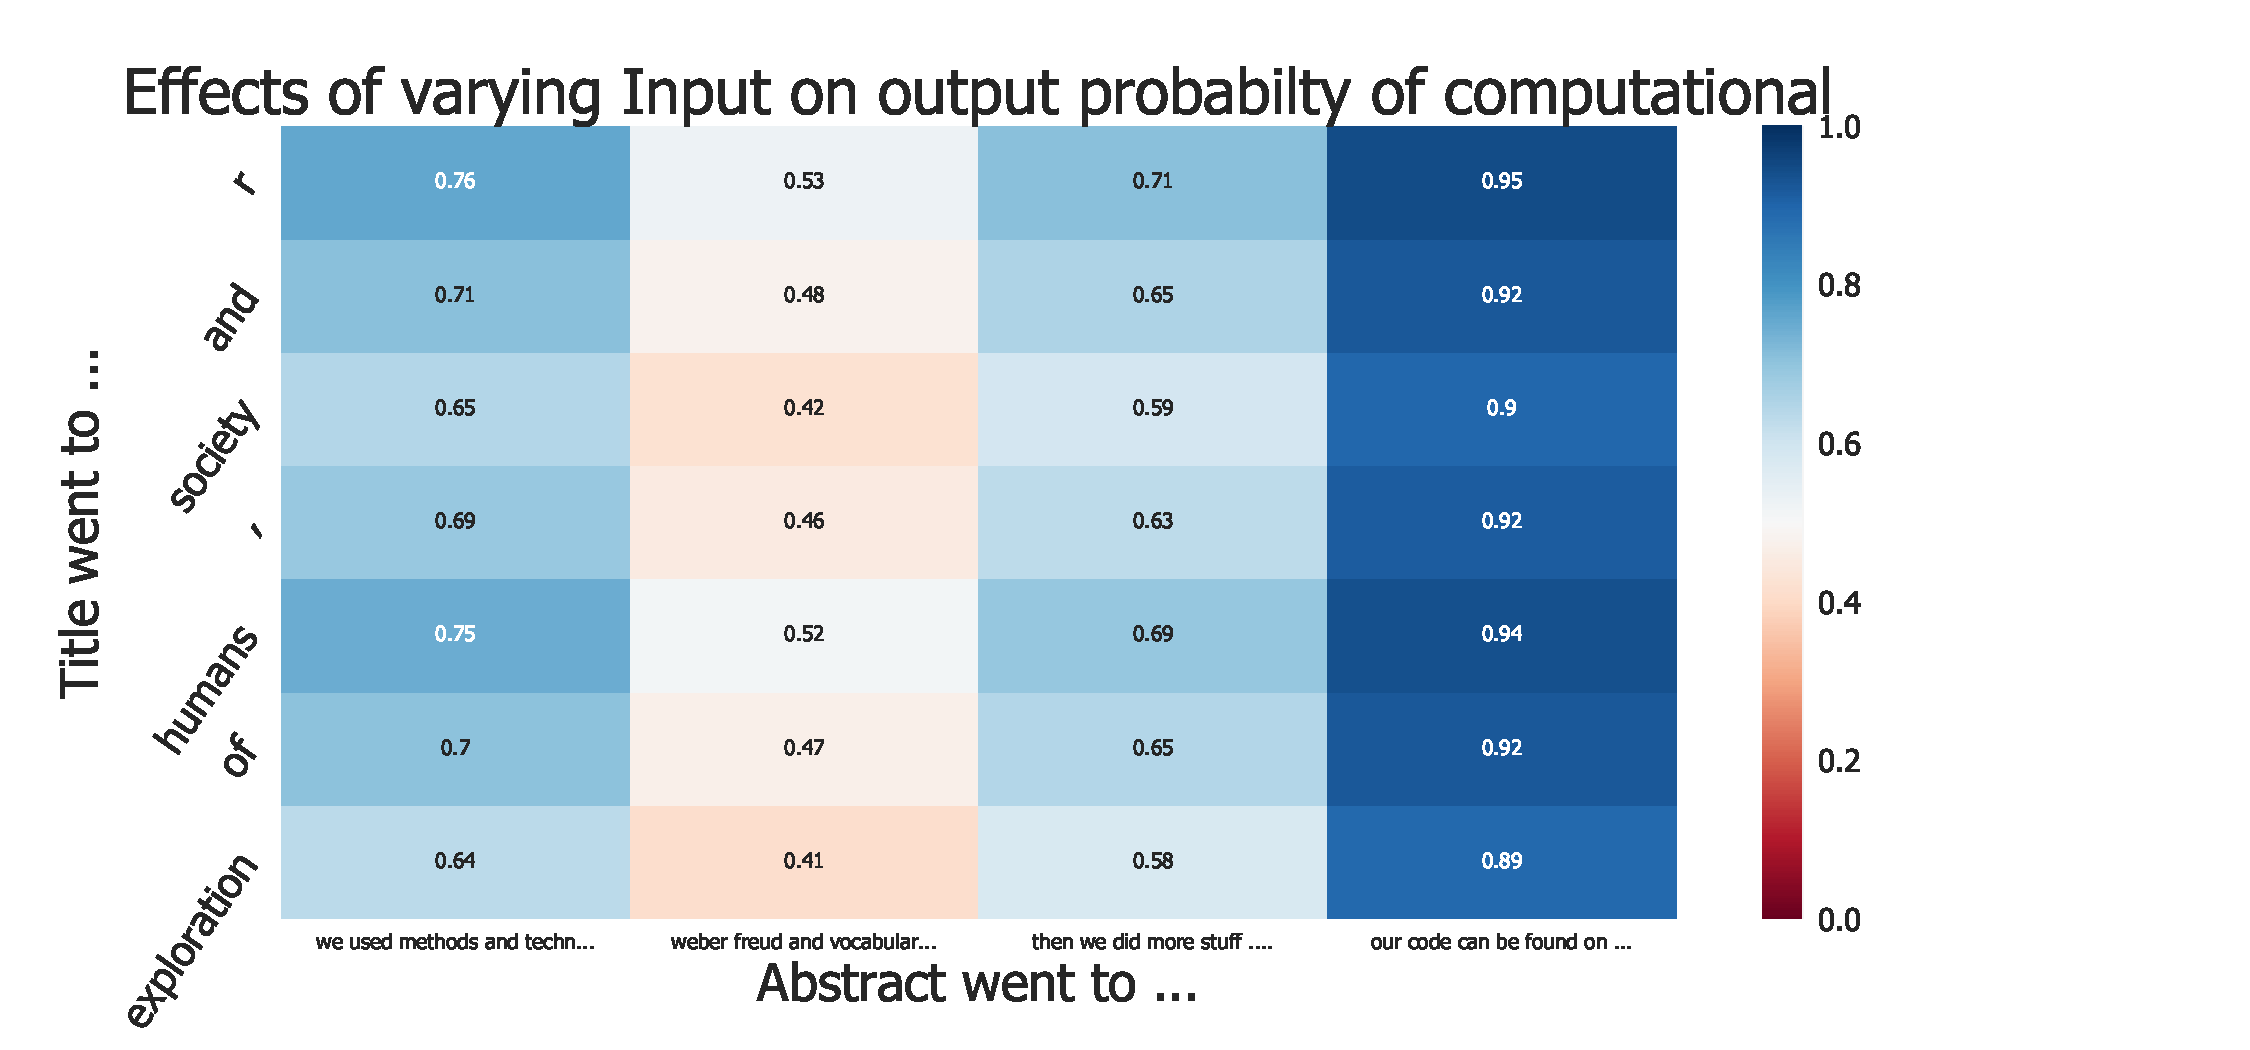
\includegraphics[width=1\textwidth]{occ_example}
	\caption{Model prediction as the title and abstract are added to, colour indicates the probability of the record being computational with blue being high and red low.}\label{oc1}
\end{figure}

\section*{Results}
\end{document}